\documentclass[twoside,10pt]{article}
\usepackage{amsmath,amsfonts,amsthm,fullpage,amssymb}
%\usepackage{mymath}
\usepackage{algorithm}
\usepackage{algorithmic}
\usepackage{graphicx}
\graphicspath{ {./} }

\begin{document}

\title{ISYE 6740 Homework 3}
%\author{Jeff Tilton}
\date{100 points total.}
\maketitle


%----------------------------------------------------------------------------------


\begin{enumerate}


\item {\bf Density estimation: Psychological experiments. (50 points)}

 The data set \textsf{n90pol.csv} contains information on 90 university students who participated in a psychological experiment designed to look for relationships between the size of different regions of the brain and political views. The variables \textsf{amygdala} and \textsf{acc} indicate the volume of two particular brain regions known to be involved in emotions and decision-making, the amygdala and the anterior cingulate cortex; more exactly, these are residuals from the predicted volume, after adjusting for height, sex, and similar body-type variables. The variable \textsf{orientation} gives the students' locations on a five-point scale from 1 (very conservative) to 5 (very liberal). %\textsf{orientation} is an ordinal but not a metric variable, so scores of 1 and 2 are not necessarily as far apart as scores of 2 and 3.
 
 \begin{enumerate}
 \item Form 2-dimensional histogram for the pairs of variables (\textsf{amygdala}, \textsf{acc}). Decide on a suitable number of bins so you can see the shape of the distribution clearly. 
 
 \begin{figure}[h]
\caption{Example of a 2 dimensional histogram with 5 bins.  Amygdala is on the x-axis and acc is on the y-axis.}
\centering
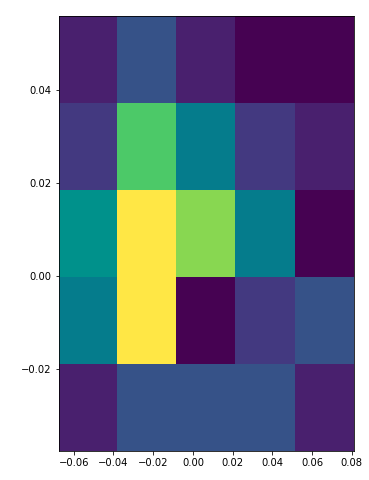
\includegraphics[width=0.5\textwidth]{1_a.png}
\end{figure}
 
 \item Now implement kernel-density-estimation (KDE) to estimate the 2-dimensional with a two-dimensional density function of (\textsf{amygdala}, \textsf{acc}). Use a simple multi-dimensional Gaussian kernel, for $x = \begin{bmatrix}x_1\\x_2\end{bmatrix}\in \mathbb R^2$, where $x_1$ and $x_2$ are the two dimensions respectively \[K(x) = \frac{1}{\sqrt {2\pi}} e^{-\frac{(x_1^2 + x_2^2)}{2}}.\] Recall in this case, the kernel density estimator (KDE) for a density is given by
 \[
 p(x) = \frac 1 m \sum_{i=1}^m \frac 1 h
 K\left(
 \frac{x^i - x}{h}
 \right)
 \]
 where $x^i$ are two-dimensional vectors, $h >0$ is the kernel bandwidth. Set an appropriate $h$ so you can see the shape of the distribution clearly. Plot of contour plot (like the ones in slides) for your estimated density.
  
 \begin{figure}[h]
\caption{Example of a 2-dimensional KDE plot using a simple Gaussian kernel with bandwidth=.0085.  }
\centering
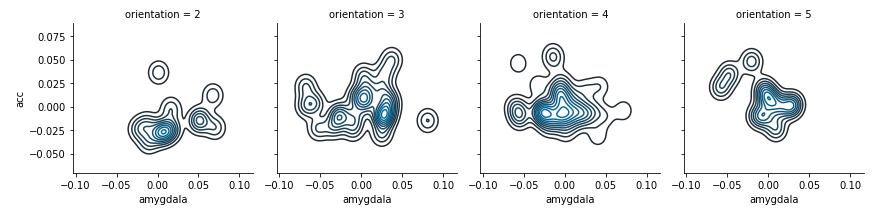
\includegraphics[width=0.9\textwidth]{1_b.png}
\end{figure}
 
 
  
 \item Plot the condition distribution of the volume of the \textsf{amygdala} as a function of political \textsf{orientation}: $p(\textsf{amygdala}|\textsf{orientation}=a)$, $a = 1, \ldots, 5$. Do the same for the volume of the 
 \textsf{acc}. Plot $p(\textsf{acc}|\textsf{orientation}=a)$, $a = 1, \ldots, 5$. You may either use histogram or KDE to achieve the goal.
\begin{figure}[h]
  \centering
  \begin{minipage}[b]{0.4\textwidth}
    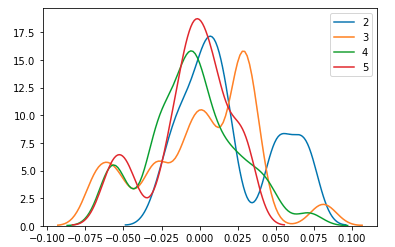
\includegraphics[width=\textwidth]{amyg.png}
    \caption{1-dimensional KDE plot using a simple Gaussian kernel with bandwidth=.0085 for the Amygdalla sample.}
  \end{minipage}
  \hfill
  \begin{minipage}[b]{0.4\textwidth}
    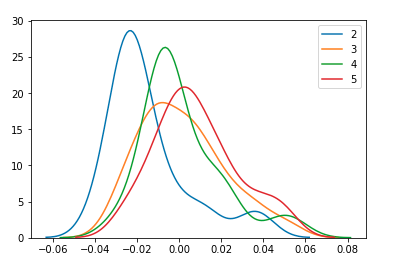
\includegraphics[width=\textwidth]{acc.png}
    \caption{1-dimensional KDE plot using a simple Gaussian kernel with bandwidth=.0085 for the Acc sample.}
  \end{minipage}
\end{figure}
 
 
 
 \end{enumerate}



\item {\bf Implementing EM algorithm for MNIST dataset. (50 points)} 

 Implement the EM algorithm for fitting a Gaussian mixture model for the MNIST dataset. We reduce the dataset to be only two cases, of digits ``2'' and ``6'' only. Thus, you will fit GMM with $C = 2$. Use the data file \textsf{data.mat} or \textsf{data.dat} on Canvas. True label of the data are also provided in \textsf{label.mat} and \textsf{label.dat}

%If you use MATLAB, you may use the following programs (see Canvas) to load the images and their labels:
%\begin{verbatim}
%images = loadMNISTImages('t10k-images-idx3-ubyte');
%\end{verbatim}
The matrix \textsf{images} is of size 784-by-1990, i.e., there are totally 1990 images, and each column of the matrix corresponds to one image of size 28-by-28 pixels (the image is vectorized; the original image can be recovered, e.g., using MATLAB code, \textsf{reshape(images(:,1),28, 28)}.


\begin{enumerate}

\item Select from data one raw image of ``2'' and ``6'' and visualize them, respectively. 

 \begin{figure}[h]
\caption{Example of a 2 and 6 hand written digit from the MNIST data set.  }
\centering
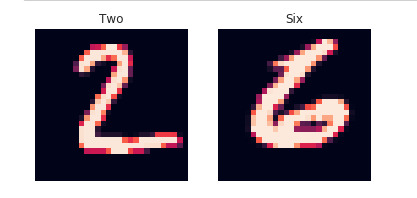
\includegraphics[width=0.5\textwidth]{2_a.png}
\end{figure}

\item Use random Gaussian vector with zero mean as initial means, and identity matrix as initial covariance matrix for the clusters. Please plot the log-likelihood function versus the number of iterations to show your algorithm is converging.


 \begin{figure}[h]
\caption{Log-likelihood per iteration of the EM algorithm where K=2 using a subset of the MNIST dataset}
\centering
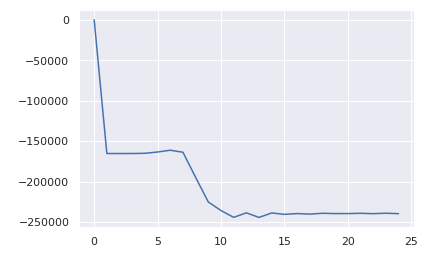
\includegraphics[width=0.75\textwidth]{2_b.png}
\end{figure}

I am not sure what I have done to invert my log-likelihood.  It is obviously decreasing instead of increasing.  I have checked my calculations and the appear correct, but I have obviously missed something.

\item  Report the finally fitting GMM model when EM terminates: the weights for each component, the mean vectors (please reformat the vectors into 28-by-28 images and show these images in your submission). Ideally, you should be able to see these means corresponds to ``average'' images.  No need to report the covariance matrices. \newline






 My ending $\pi_k$ values were 7.76e-09 and 2.74e-08 respectively, average images are seen below.
 
 It is interesting to compare the images to the plot of log-likelihood.  There is little to no change between iteration 2 and 7, then just a slight improvement in the log-likelihood corresponds to finally being able to distinguish the separate numbers in iteration 8.  Then there is not much visual difference between iteration 9 and the final iteration, although there was significant improvement in the log-likelihood.

 \begin{figure}[h]
\caption{Average of the 2 clusters for chosen iterations.}
\centering
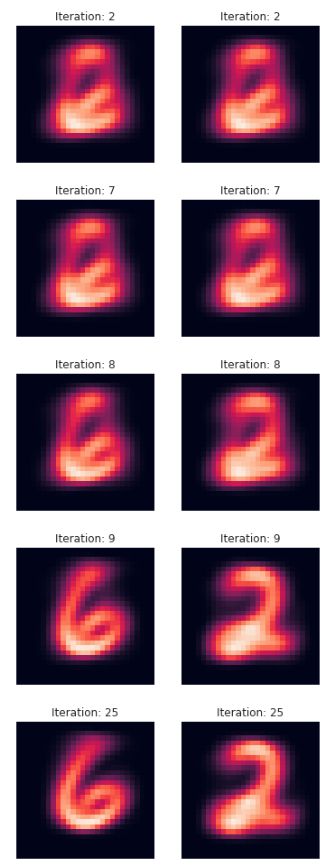
\includegraphics[width=0.35\textwidth]{2_c.png}
\end{figure}

\end{enumerate}

\end{enumerate}

\end{document}
